\RequirePackage{fix-cm}
\documentclass[11pt,twocolumn,letterpaper]{article}
\usepackage[fontsize=10.5pt]{scrextend}

\usepackage{cvpr}
\usepackage{times}
\usepackage{epsfig}
\usepackage{graphicx}
\usepackage{amsmath}
\usepackage{amssymb}
\usepackage{subfig}
\newcommand{\norm}[1]{\left\lVert#1\right\rVert}

% Include other packages here, before hyperref.

% If you comment hyperref and then uncomment it, you should delete
% egpaper.aux before re-running latex.  (Or just hit 'q' on the first latex
% run, let it finish, and you should be clear).
\usepackage[breaklinks=true,bookmarks=false]{hyperref}
\graphicspath{ {./images/} }
\cvprfinalcopy % *** Uncomment this line for the final submission

\def\httilde{\mbox{\tt\raisebox{-.5ex}{\symbol{126}}}}

% Pages are numbered in submission mode, and unnumbered in camera-ready
%\ifcvprfinal\pagestyle{empty}\fi
\setcounter{page}{1}
\begin{document}
%%%%%%%%% TITLE
\title{Employing Ensemble Learning Techniques to Create a Modular and Updatable DeepFake Detection Model}

%%%%%%%%% AUTHORS
\author{Rengang Yang\\
Texas A\&M University\\
College Station, TX\\
{\tt\small ry3956@tamu.edu}
\and
Zengxiaoran Kang\\
Texas A\&M University\\
College Station, TX\\
{\tt\small zk2487@tamu.edu}
}
\maketitle

%%%%%%%%% ABSTRACT
\begin{abstract}
Since the advent of Generative Adversarial Networks (GANs), the DeepFake community has exploded in popularity and has become a point of contention in politics and society. The increase in activity has spawned many generators based on GAN (ProGAN, StyleGAN, BigGAN, etc.), which are well documented and easy to use. As a result, most of the research on DeepFake detection has jumped straight to Deep Neural Networks (DNNs). This approach allows them to make monolithic all-in-one models to detect forgeries of any generator, but often come with significant downsides. We propose, instead, to take a more modular approach, using techniques borrowed from Ensemble Learning. By having dedicated models trained to the output of individual generators, we can effectively use patterns left by individual generators that are not utilized in DNNs. Then, this data can be aggregated by vote, and effectively capture overarching patterns as well as minutiae. Our goal is to evaluate whether such a system can be more efficient in training as compared with DNNs, while also being as accurate. 
\end{abstract}

%%%%%%%%% BODY TEXT
\section{Introduction}
The development of image generators has been accelerating at an elevated pace, and there exists a lot of concern from large players over its ethical uses. To combat this, the development of Fake Image classifiers have been backed with millions of dollars from large companies like Google, Facebook, and Microsoft \cite{stateOfDeepFakes}, as well as government bodies \cite{stateOfDeepFakes}. To this end, as the field has not stabilized, the game of cat-and-mouse between detectors and generators is still accelerating, with generators now being made to take into account detectors \cite{neekhara2020adversarial}. 
We believe that this rapid pace of change, combined with targeted development from the image generators, mean that fake image detectors need to be able to adapt to new algorithms as they come out, or else they would be ineffective against such changes. By having as many generators represented through, individual specialized models, we can effectively capture features or idiosyncrasies of specific generators, on a level that a DNN would struggle to be computationally viable \cite{sze2017efficient}. This is before mentioning the vulnerability to adversarial attacks that is inherently part of using a DNN \cite{neekhara2020adversarial}. \par
Here, we propose our two-part approach to tackle the problem of identifying fake images through a modular approach. The first part, main classification model, is trained to attempt to classify what image generator it might think a sample image was generated with. The confidence values outputted from that first model then would become the weights to augment the prediction the second part, the ensemble learning. The final value, as a sum of the individual predictions multiplied by the known weights, will classify whether an image is fake or real. Many individualized models are made for as many specific generators as the main model can classify, and they vote based on weights determined from before. \par
We establish that we can first use linear SVMs \cite{10.1145/130385.130401} \cite{10.1023/A:1022627411411} as our base model, as they are one of the most widely used non-NN non-linear classifiers, when the data is labeled. In order to keep any bias out, as well as reduce the possibility of overfitting the data, we will generate our own data from seed data that companies specifically developed for this task \cite{rssler2019faceforensics}, before testing performance (not validation) on a publicly available dataset, like the one developed by AWS, Microsoft, and Facebook. Our testing is limited to image generators open to the public, and perhaps could be weak against closed-source or completely private generators. \par
However, we still believe that it would be simpler to train and setup compared to a DNN. The tradeoff in flexibility can be made up by the ability to massively parallelize the training procedure, and the ability to update for new developments without major code overhaul or retraining. \par

\begin{figure*}
    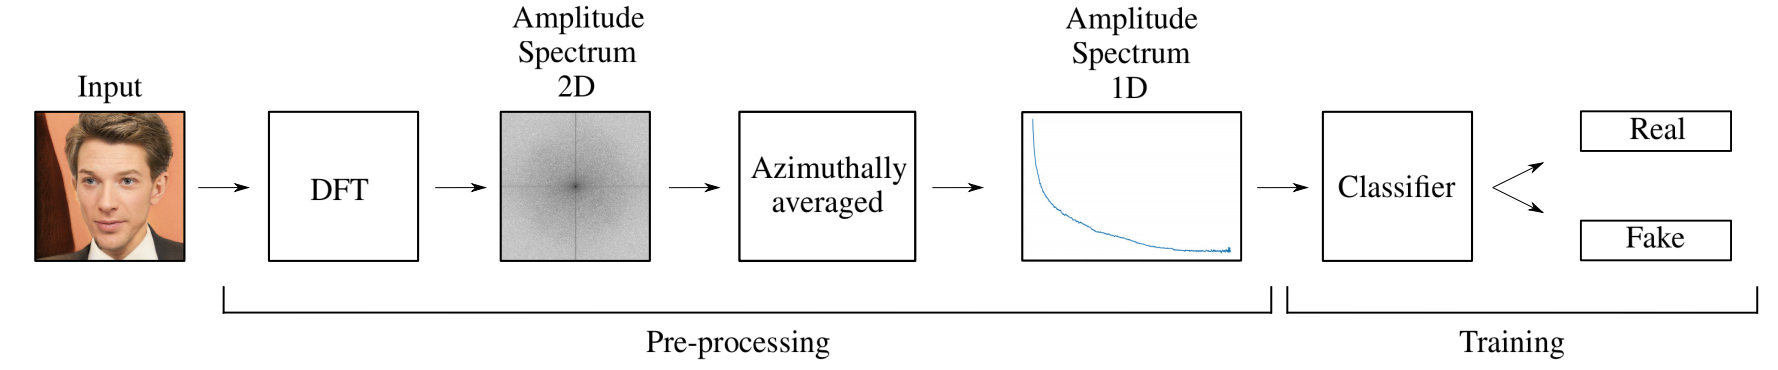
\includegraphics[width=\textwidth]{preprocessing-pipeline}
    \caption{Main overview of the preprocessing pipeline. The image is processed through feature extraction using DFT, and then the classifier is trained on the processed data.}
\end{figure*}
% old introduction ended here.
Since 2017, the techniques of Deep Fakes have developed and grown rapidly in various industries globally. However, due to the significance on societal and political impact followed by its growth of technical sophistication \cite{stateOfDeepFakes}, many detection algorithms have been necessarily developed to classify whether products are deepfake-generated. In general, there were three types of classification targeted on images, audio, and videos, primarily applying the neural network techniques like DNNs and RNNs. \par
We note that most new generators come from the development of either Variationally Autoencoders (VAE)\cite{kingma2013autoencoding}, or Generative Adversarial Networks (GAN)\cite{goodfellow2014generative}. GANs, in particular have seen an acceleration in development since its groundbreaking debut. \cite{brock2018large}\cite{karras2017progressive}.\par
Despite this accelerated development in terms of image generation, fake detection has not been keeping up. Most of the current classifiers usually will fall into one of two categories: neural networks designed to be a generalized solution or relatively complicated pre-processing fed into non-NN learning techniques. We have found that most DNN based solutions have inherent issues with handling adversarial attacks \cite{neekhara2020adversarial}. Despite this, they are still the most accurate and thus our main focus will be on the comparison with Convolutional Neural Network (CNN) approaches by Amerini et. al \cite{Amerini_2019_ICCV}, and by Li and Lyu \cite{li2018exposing}. We will also be testing with Durall et. al with their method of Discrete Fourier Transformations as a preprocessing step \cite{durall2019unmasking}. These approaches are understood to be state-of-the-art as of the writing of this paper. \par
The approach we considered for our application was Ensemble Learning, which includes SVM, PCA, and other non-DNN approaches. We want to note that many of the preprocessing techniques shown by Durall et. al \cite{durall2019unmasking} are also be applied per-generator. For future work, we may use the method described by Guera and Delp \cite{Guera2018DeepfakeVD} to extract useful features when handling videos. Mantern et. al \cite{Matern2019ExploitingVA} suggests an interesting method detecting images GANs and VAE. This approach detects the difference in eye color (the highly contrasted pixels between Iris and sclera) by comparing and calculating the HSV value of the left and right eyes. However, all the approaches above target one specific anomaly or inconsistency resulting from the production of deepfake production, that with updates can be taken account for. We have already seen this happen, where anomaly-based detection schemes are made obsolete by updates to generators \cite{neekhara2020adversarial}. Thus, having the ability to adapt the model without having to completely retrain is useful.

\section{Methods}
In this section, we will discuss our experiment in terms of the linear SVM models we used, as well as the other data processing steps that were taken.

\subsection{Data Pre-processing}
There were two main steps that we used in order to be able to numerically quantify the visual data. One of the ideas is Discrete Fourier Transformations, which is well known in computer vision. The other step, Azimuthal Averaging, was a technique utilized by Durall et al. in their experiment to decompose the differences out of generated imagery. \cite{durall2019unmasking}

\subsubsection{Discrete Fourier Transformations}
The Fourier Transformation is a mathematical analysis technique which can decompose a function into its constituent frequencies. Especially for computer vision, this technique is able to detect the repetitive features of images, such as analyzing the frequency of pixel signals being distributed in the frequency domain power spectrum. It is widely implemented in image application and processing, such as image filtering, image compression, and image reconstruction. 
$$ X_k = \sum^{N-1}_{n=0} X_n * e^{- \frac{2 \pi i}{N} kn} $$
$$ = \sum^{N-1}_{n=0} X_n * [\cos(\frac{2\pi k n}{N}) - i * \sin(\frac{2 \pi k n}{N})] $$ \par
In this experiment, we implement the discrete version of Fourier Transform to decompose the image files into its sine and cosine components in the Fourier or frequency domain. The output image is spatially equivalent to the input image which in practice reveals more information from the intensity variation of pixels undergoing the change. This also means that the equation needs to be implemented for a 2d image, as such:
$$X_{k, l} = \sum^{N-1}_{n=0} \sum^{M-1}_0 x_{n, m} * e^{\frac{2 \pi k n}{N}} * e^{\frac{2 \pi l m}{M}} $$
The output image will represent the amplitude and phase of the signal at each pixel. It should be noted that there has been considerable research into defending against this processing step. \cite{zhang2019adversarial}\par
This step is also important in that it allows us to significantly decrease the storage and computational needs of the system. While it was not tested in our system, this preprocessing step could be done on an edge device before being sent to a central server to compute. The development of fast Fourier transforms, like FFT (fast Fourier transform) allow this to be done as fast as data ingestion allows, or real-time \cite{zeman2019discrete}.

\begin{figure}%
    \centering
    \subfloat[Original Image]{{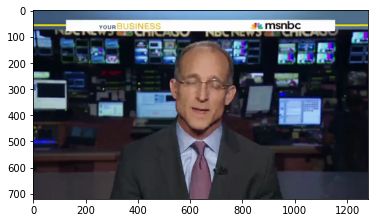
\includegraphics[width=3.5cm]{before} }}%
    \qquad
    \subfloat[Image with DFT]{{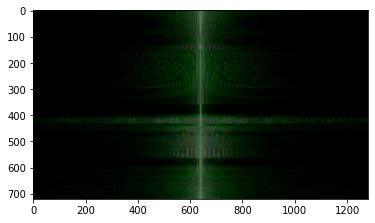
\includegraphics[width=3.5cm]{after} }}%
    \caption{Image before and after Discrete Fourier Transformations. This image was not cropped, but in our experiment, all images where cropped to be the center square.}%
    \label{fig:example}%
\end{figure}

\subsubsection{Azimuthal Average}
In order to create a robust representation of the image in 1D, azimuthal averaging can be used on the Fourier Transformation power spectrum. In this case, it is similar to compression. The value at each pixel is redefined as the arithmetic mean of the pixel located on a radius along a defined annulus of that radius centered on the image. After applying a Fourier Transformation, the output image presents in a frequency domain that has the same dimensionality and property as the spherical coordinate system. Under a similar system, we can apply azimuthal averaging to further improve the robustness and performance of Fourier-transformed images without losing much relevant information. 

\subsection{Classification Algorithms}
\begin{figure*}
    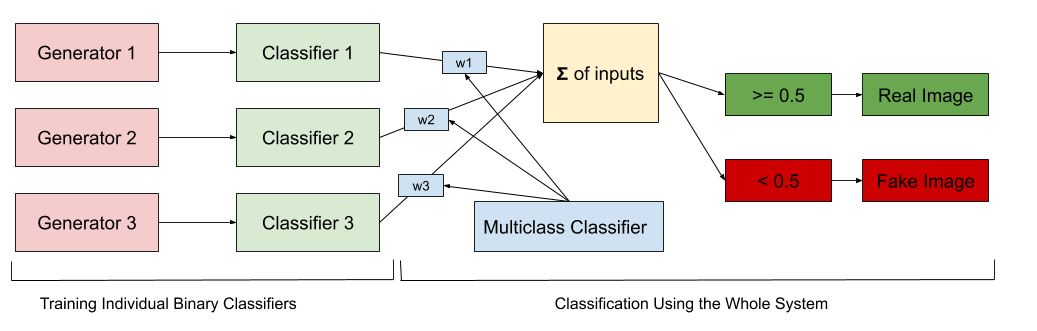
\includegraphics[width=\textwidth]{Classification-Pipeline}
    \caption{Main overview of the Classification pipeline. The classifiers 1-3 are trained to the outputs of one specific generator. In our case, we used DeepFake, Face2Face, and Faceswap as our generators. The latter half uses the model to classify images.}
\end{figure*} 
Our goal was to not use any neural-network based algorithms, due to the complexity that they bring as well as the vulnerability they have against adversarial attacks. Our testing will specifically focus on the SVM implementation, as that is the only algorithm we had time to fully tune and train. As such, while we will discuss possible implementations using K Means, along with potential benefits it can bring, it was not verified in our work through testing. All testing results will only refer to SVMs.

\subsubsection{Support Vector Machines}
Support Vector Machine (SVM) is a well-known popular supervised machine learning algorithm suitable for binary non-linear classification problems with strong mathematical support\cite{10.1145/130385.130401} \cite{10.1023/A:1022627411411}. 
$$\text{Minimize: } J(w, b, a) $$
$$= \frac{1}{2} w^T w - \sum^{N}_{i=1} a_id_i(w^Tx_i + b) + \sum^N_{i=1}a_i$$
$$\text{Subject to: } a_{i} \geq  0\text{ } \forall \text{ } i$$
\par
The general objective of SVM is to identify the optimal boundary or hyperplane that maximizes the marginal between two support vectors from different classes. We used a soft-margin version of SVM to compromise unpreventable small errors from the noise of image data. In SVM, the loss function is hinge loss. That is, as the previous formula indicates, will only punish the weights if the classifier is wrong and none otherwise. Given a set of training pairs ($x_i, y_i$), where $x_i \in R_n$ and $y_i \in {1, -1}$. The solution for SVM is to optimize:
$$\text{max } \sum^{m}_{i=1} \alpha_i - \frac{1}{2}\sum^m_{i=1}\sum^m_{j=1}\alpha_i\alpha_jy_iy_j x_ix_j $$
$$\text{s.t. } 0 \leq \alpha_i \leq C $$
$$\sum^m_{i=1}\alpha_iy_i = 0$$\par 
In our work, we used the gaussian kernel to map vectors $x_i$ into a higher dimensional space in order to conquer some non-linearity data.
\subsubsection{K Means}
We also want to attempt unsupervised learning on given subjects. Hence, we choose K-Means Clustering algorithms and measure the score of detection without giving labels to the dataset. K-Means clustering is an exploratory data analysis method that aims to cluster similar data points together. The cost function and the gradient descent function is given below. The algorithm tries to find homogeneous subgroups by iteratively calculating the Euclidean distance of each feature from the initial centroids $\mu$ to identify nearby features. The identified features will be assigned to the closest centroid and new centroid sets will be recalculated with the new identified features in each round of iteration.  We can determine the number of classification by a given K number of clusters. 
$$J = \sum^m_{i=1} \sum^K_{k=1}w_{ik}\norm{x^i - u_k}^2$$
$$\frac{\partial J}{\partial w_{ik}} = \sum^m_{i=1} \sum^K_{k=1} \norm{x^i - u_k}^2$$
\[ \Rightarrow w_{ik}= \begin{cases} 
    1 & \text{if } k = argmin_j \text{ } \norm{x^i - \mu_j}^2 \\
    0 & \text{otherwise.}
 \end{cases}
\] \par
The strength of K-Means in this case mostly lies in its ability to learn unsupervised. This could be useful for large datasets that haven't been manually verified like ours has been, but comes with the usual detriments that K-Means comes with: The slow prediction times as well as the initialization problem.

\section{Experiment}
In this section, we show the result of our experiment and evaluation of our approach. We will first introduce a high resolution dataset FaceForensics++ \cite{rssler2019faceforensics}, then describe our training pipeline and settings, and finally discuss our experiment result in detail. 

\begin{figure*}
    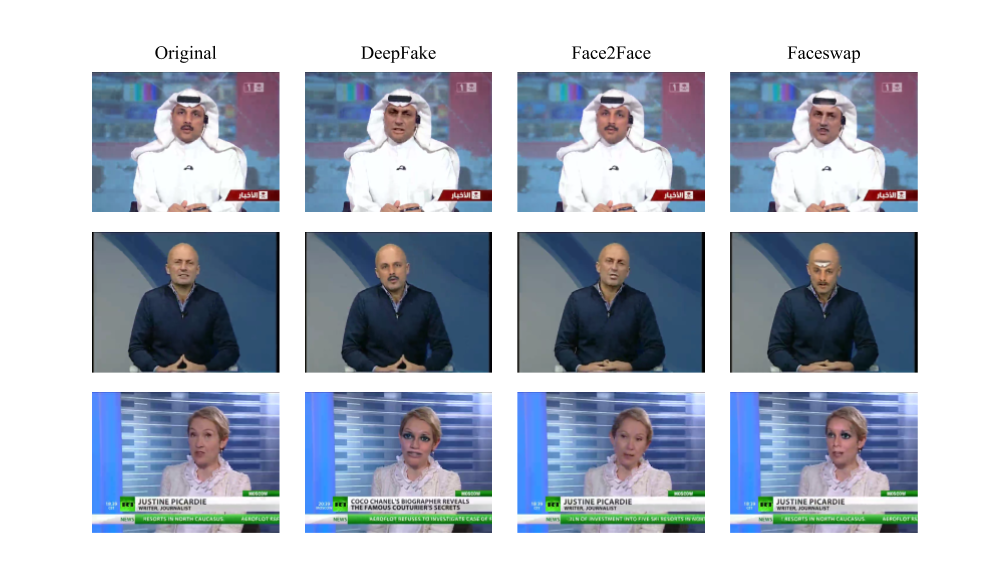
\includegraphics[width=\textwidth]{example-data}
    \caption{Peek into the dataset that we used. FaceForensics++ data was fed into three of the most user accessible generators available, and this was used to create the training sets}
    \label{fig:dataset}
\end{figure*} 
\subsection{Dataset}
In this experiment, we downloaded our image files from FaceForensics++ dataset, made available by Andreas Rössler in conjunction with Google. This dataset consists of 1,000 original unmodified videos scraped from the web. The data has been sourced from 977 YouTube videos and all videos contain a trackable mostly frontal face without occlusions which enables automated tampering methods to generate realistic forgeries. These videos were then used to produce altered videos using 4 common generators: DeepFake, Face2Face, Faceswap, and NeuralTextures. Each generator created 1,000 video sequences, though we did not end up using NeuralTextures due to its high degree of similarity to DeepFake.\par
We extracted frames from the given videos and imported them with label 0 as fake and 1 as real into a huge sample pool. Due to the size of the dataset, we used the highest compression setting available to us, but the extracted images still took up around 2.2TB of space. For ease of recreation, we have included the processed and pickled data in our repository.


\subsection{Processing Data}
The pre-process of images contain two parts. First we take the entire dataset and transform every sample image to a spatial domain and then to a 1D frequency domain, converting 1024x1024x3 high-quality color video frames cropped to 722 features (1D Frequency Domain Power Spectrum). This method is being introduced in the previous method section, a combination of Discrete Transform Formula and Azimuthal Averaging. The transformation is substantially optimized by a built-in python numpy package and hence provides very robust information without losing too much content.
Since the images are cropped from video files and their sizes may vary, we added an extra process before the classifier that interpolates the 1D Power Spectrum to a fixed size (N = 300) and normalizes it dividing it by the 0th frequency component.\par
After data preparation, we select the Radial Basis Kernel (RBF) \cite{JMLR:v11:chang10a} for the SVM model and the optimal tuning parameters we choose are gamma = 0.86 and c = 6.37. These values were selected after multiple small sample runs, and we determined that it offered the highest probability of convergence. The RBF is a popular kernel function taking two sample data  x and x' represented feature vector in another input space defined as below.
$$K(x, x') = e^{-\frac{\norm{x-x'}^2}{2\sigma^2}}$$


\subsection{Power Spectrum}
\begin{figure}%
    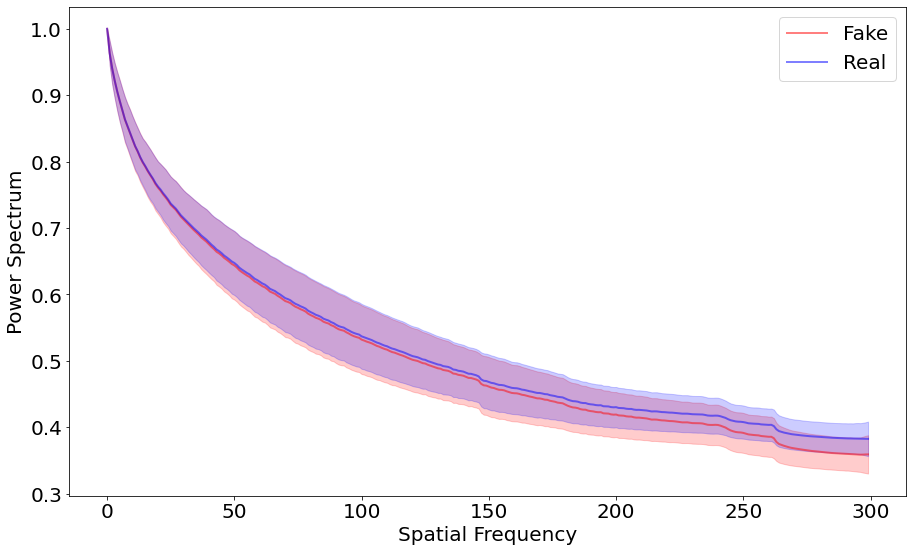
\includegraphics[width=8cm]{power-spectrum}
    \caption{Power spectrum showcasing the difference between the real and fake images after the pre-processing steps.}
    \label{fig:power-spectrum}
\end{figure}
As shown in Figure \ref{fig:power-spectrum}, fake images will have different frequency characteristics. Despite overlapping similarities in the purple region, there is a clear and distinguished difference between the real and the fake images. The offset has a positive correlation with the spatial frequency. We use this offset to perform classification. However,the purple region also indicates that there will be some overlap. We hope that with some tuning, the kernel trick in SVM will further differentiate the values, and provide a solid classification result. Our model in theory will not perform well on low-resolution images. On the other hand, this method will show better performance with medium-high resolution images. The given input with higher resolution will result in a bigger gap in offset as its spatial frequency increases; hence, it will be clearer to be classified with our model.

\subsection{Binary Classifiers}
Here, we examine the properties of our binary classifiers standalone. They will only be tested on data generated by the generator they are against. Rather than using a typical convolutional neural network to extract features from images, we sample features by converting image data into Frequency Domain Power Spectrum. Our approach is based on a high-frequency component analysis. This method is expected to have relatively poor performance in low-resolution images due to limited spam of the frequency spectrum. For medium and high resolution deepfake images, the method has well-performed robustness. \par
Our classifiers were trained on a dataset comprised of 50/50 fake and real images. We used a 10,000 dataset size, that is, 10,000 each of fake and real images to train the generator. We also had to do multiple tests to tune hyper-parameters in terms of cleaning data. \par
Our result indicates that the preprocessing step is capable of detecting fake images on Forensic Face++ dataset with around an 80\% successful rate. This data is more or less in-line with similar but more extensive experimentation done by Durall et al \cite{durall2019unmasking}. However, our dataset was considerably more compressed, which affected overall effectiveness.\par
As an aside, we found that the binary classifiers were able to also classify other generators data surprisingly well (70-75\% accuracy), and we believe that it is due to the similarities that underlie most of the generators we are testing. Only Face2face \cite{thies2016face}, which was not based off of DeepFake and GANs, had significantly worse classification results when using classifiers trained on the output of the other two generators.
\begin{table}[h]
    \centering
\begin{tabular}{|l|c|}
\hline
Generator & Accuracy \\ \hline
DeepFake  & 83\%     \\ \hline
Face2Face & 79\%     \\ \hline
Faceswap  & 82\%     \\ \hline
\end{tabular}
\end{table}

\subsection{Multiclass Classifier}
The multiclass classifier, used to determine which class it thought it was, ended up being the SVM again. In our configuration, which we used scikit-learn's built in Support Vector Classifier, uses a one-vs-one system in order to extend SVM into a multiclass classifier\cite{Smola04atutorial}\cite{scikitlearnSVC}. We again used the gaussian RBF kernel function that it defaults to, though we did test on other kernel functions that were offered. We did not find any tangible improvements in accuracy when changing to either linear or sigmoid, and thus stuck with RBF.\par
Admittedly, this is where the project did not perform up to expectations.
\begin{figure}%
    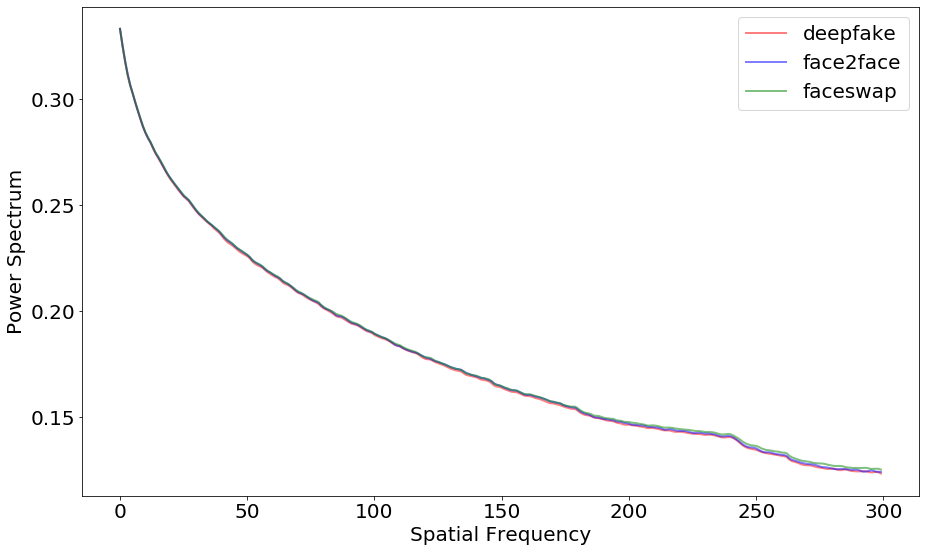
\includegraphics[width=8cm]{multiclass-power-spectrum}
    \caption{Power spectrum when classifying between multiple types of generated data}
    \label{fig:mult-power-spectrum}
\end{figure}
We can see in Figure \ref{fig:mult-power-spectrum} that the spectrum is much closer than classifying between real and fake. There is little differentiation between them, and thus it ended up with a 45\% accuracy rate. However, despite this low level of success, we found that because it's confidence values between the three classifiers were relatively similar, this could effectively be used as a regularizer. If an outlier, or clearly obvious fake from one generator appears, the multiclass will give preferential weighting to that binary classifier. Likewise, if a real photo appeared or fake images generated from other generators not tested here, it would roughly equally weight it between all generators. This is relevant because we intentionally trained it to not classify real data, as that is the job of the binary classifiers. In essence, this classifier is used as a way to point to which binary classifier it thinks is best.

\subsection{Combined Ensemble Classifier}

\begin{table}[h]
    \centering
\begin{tabular}{|l|c|}
\hline
Generator & Accuracy \\ \hline
DeepFake  & 91\%     \\ \hline
Face2Face & 84\%     \\ \hline
Faceswap  & 89\%     \\ \hline
Fake(avg) & 88\%     \\ \hline
Real      & 94\%     \\ \hline
\end{tabular}
\end{table}\par
We can see from the above table that when the ensemble classifier was created, it did boost the performance of the generators a not-insignificant amount. It was actually quite interesting to see how it was much better at classifying real data as real than it was the other way around. The individual accuracies also closely relate to the original binary SVM accuracies. Likewise, as we expected, Face2Face is much harder to classify, as that is both visually true (Figure \ref{fig:dataset}), as well as the difference in underlying technology. It should be noted that all accuracy scoring was done using the scikit-learn built in scoring function. To make the scoring more applicable to the real world, one can instead look at true positive rates or true negative rates, and determine which is more important to them in their specific application.\par

\section{Conclusion}
In this experiment, we attempted to classify images generated from DNNs in a way that doesn't require neural networks. We first preprocessed the image using Discrete Fourier Transforms, before Azimuthally averaging the data to obtain a one-dimensional amplitude spectrum that we can then run our selected classification algorithms on. We applied Support vector machines, for it's robustness and known ability to classify non-linear data in both the binary and multiclass cases, on a dataset generated using DeepFake, Face2Face, and Faceswap on the Faceforensics++ original dataset.\par
Our model achieved great accuracy in our testing on the Faceforensics++ dataset, we understand that a lot of it is due mostly to how well prepared the data is. All the videos available in the dataset was checked by hand by Rössler et al \cite{rssler2019faceforensics}, and cleaned in a way that the image artifacts that appear during the image manipulation process is maximized. There is no guarantee that the data will be anywhere as clean or as uniform as in our test set. Likewise, without face detection software, we rely on the image to be already centered on human faces, which isn't always the case. Better centering on faces could potentially lead to better results, as it would discard much of the unnecessary data that surrounds the image. We also found that the multiclass classifier that we trained didn't offer as much of a boost in performance as we had hoped it would, and anecdotally, it could be removed and simply using the average of the multiple binary classifiers would have been just as accurate.\par
As an aside, we want to acknowledge the continuous work that goes on in deepfake generation. We chose the generators DeepFake, Faceswap, and Face2Face due to its maturity in end user software, as well as ease of use due to pre-trained models, but these are no longer cutting edge. Since the proposal of this paper, we note that newer techniques have been developed to significantly reduce the difference we would see in the power spectrum \cite{dang2019detection} \cite{tolosana2020deepfakes}. Likewise, our small sample-size of generators was due mostly to our limited time and computing resources.

\section{Future Discussion}
Surprisingly, or perhaps unsurprisingly, we don't recommend a continuation of our route. While non-DNN solutions do exist and continue to exist, generators have been out-pacing development of image processing techniques to find deepfakes. In the end, the best way to classify a DNN generated image is to also have an extensively trained DNN. For that route, it would better to move the route of Huang et al \cite{Huang2020FakeLocatorRL}, as they achieved better results than we did on a larger amount of generators using a single RNN.

\section{Task Assignment and Acknowledgement}
This project was completed by Rengang Yang and Zengxiaoran Kang, under the instruction of Dr. Zhangyang (Atlas) Wang and Zhenyu Wu. Rengang Yang was responsible for training and tuning hyper-parameters for the classifiers used in this experiment, while Zengxiaoran Kang worked on image manipulation and data generation. Dataset creation and image processing were done collaboratively worked in Google Colaboratory. The dataset was provided by FaceForensics++. 


{\small
\bibliographystyle{ieee_fullname}
\bibliography{egbib}
}

\end{document}
